\documentclass[border=6pt]{standalone}
\usepackage{tikz}
\usetikzlibrary{arrows.meta,calc,positioning}
\begin{document}
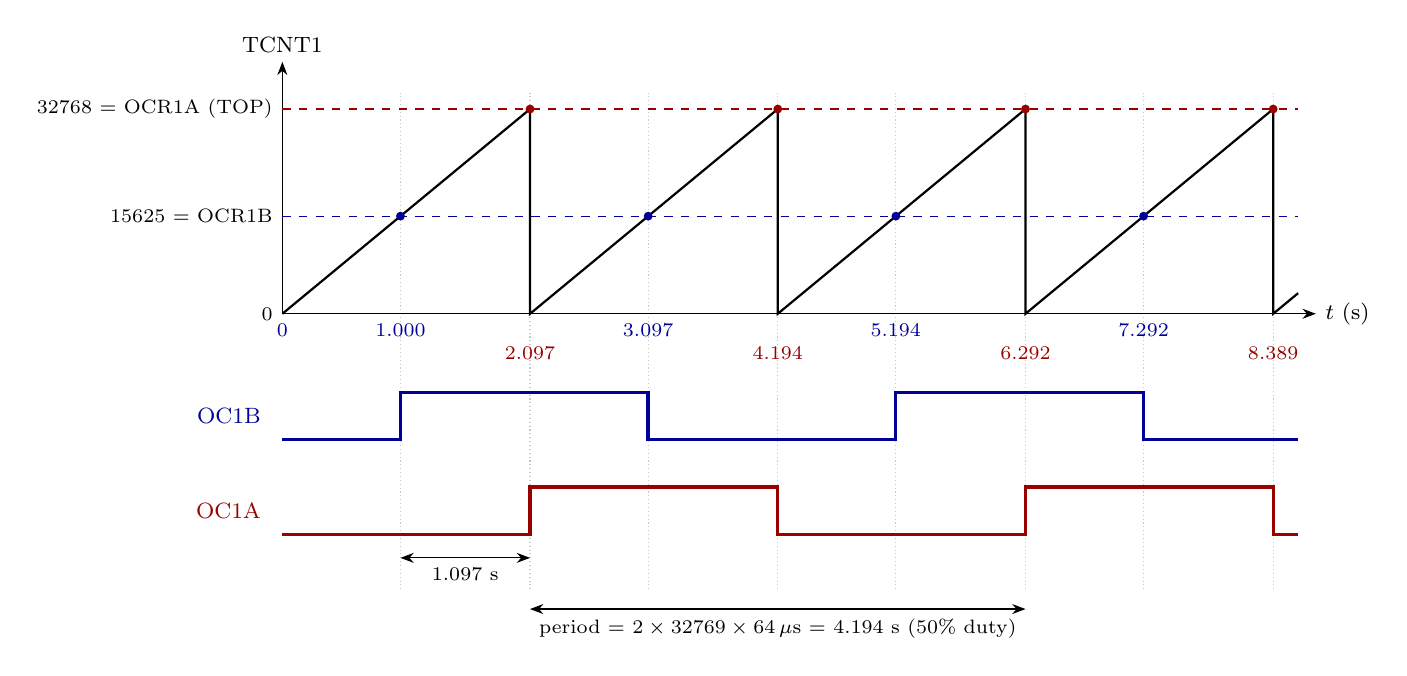
\begin{tikzpicture}[>=Stealth,font=\small,x=1.5cm,y=1cm]
% 1 unit = 1 s; 1 tick = 64 us; cycle = 32769 ticks = 2.097216 s
% OCR1B match at 15625 ticks = 1.000 s after each restart; OCR1A (TOP) match at 32768 ticks = 2.097152 s
\def\H{2.6}% 32768
\def\B{1.2397}% 15625 -> 2.6*15625/32768
\def\T{2.097216}
\foreach \t in {1.0,2.097,3.097,4.194,5.194,6.292,7.292,8.389} \draw[gray!45,densely dotted] (\t,-3.5) -- (\t,\H+0.2);
\draw[->] (0,0) -- (0,\H+0.6) node[above,font=\footnotesize]{TCNT1};
\draw[->] (0,0) -- (8.75,0) node[right,font=\footnotesize]{$t$ (s)};
\node[anchor=east,font=\scriptsize] at (0,\H) {32768 = OCR1A (TOP)};
\node[anchor=east,font=\scriptsize] at (0,\B) {15625 = OCR1B};
\node[anchor=east,font=\scriptsize] at (0,0) {0};
\draw[red!60!black,dashed] (0,\H) -- (8.6,\H);
\draw[blue!60!black,dashed] (0,\B) -- (8.6,\B);
\draw[thick] (0,0) \foreach \k in {1,2,3,4} { -- (\k*\T,\H) -- (\k*\T,0) } -- (8.6,{\H*(8.6-4*\T)/\T});
\foreach \k in {0,1,2,3} {
  \fill[blue!60!black] (\k*\T+1.0,\B) circle (1.6pt);
  \fill[red!60!black] (\k*\T+\T,\H) circle (1.6pt);
}
\foreach \t/\l in {0/0,1.0/1.000,3.097/3.097,5.194/5.194,7.292/7.292} \node[below,font=\scriptsize,blue!60!black] at (\t,0) {\l};
\foreach \t/\l in {2.097/2.097,4.194/4.194,6.292/6.292,8.389/8.389} \node[below,font=\scriptsize,red!60!black] at (\t,-0.3) {\l};
% OC1B
\begin{scope}[yshift=-1.6cm]
\node[anchor=east,font=\footnotesize,blue!60!black] at (-0.1,0.3) {OC1B};
\draw[very thick,blue!60!black] (0,0) -- (1.0,0) -- (1.0,0.6) -- (3.097,0.6) -- (3.097,0) -- (5.194,0) -- (5.194,0.6) -- (7.292,0.6) -- (7.292,0) -- (8.6,0);
\end{scope}
% OC1A
\begin{scope}[yshift=-2.8cm]
\node[anchor=east,font=\footnotesize,red!60!black] at (-0.1,0.3) {OC1A};
\draw[very thick,red!60!black] (0,0) -- (2.097,0) -- (2.097,0.6) -- (4.194,0.6) -- (4.194,0) -- (6.292,0) -- (6.292,0.6) -- (8.389,0.6) -- (8.389,0) -- (8.6,0);
\draw[<->] (1.0,-0.3) -- (2.097,-0.3) node[midway,below,font=\scriptsize]{1.097 s};
\draw[<->] (2.097,-0.95) -- (6.292,-0.95) node[midway,below,font=\scriptsize]{period = $2\times32769\times64\,\mu$s = 4.194 s (50\% duty)};
\end{scope}
\end{tikzpicture}
\end{document}
